\documentclass[handout]{beamer}
%\documentclass[presentation]{beamer}

\usecolortheme{Imperial}
 
\usepackage[utf8]{inputenc}
\usepackage[UKenglish]{babel}
\usepackage{booktabs}
\usepackage{caption}
\usepackage{subcaption}
\usepackage{graphicx}
\usepackage{amsmath}
\usepackage{amsfonts}
\usepackage{amssymb}
\usepackage{epstopdf}
\usepackage{lipsum}
\usepackage{pgfplots}
\pgfplotsset{compat=1.14}
\usepackage{enumitem}
\usepackage{xcolor}
\usepackage{multirow}

% complying UK date format, i.e. 1 January 2001
\usepackage{datetime}
\let\dateUKenglish\relax
\newdateformat{dateUKenglish}{\THEDAY~\monthname[\THEMONTH] \THEYEAR}

% Imperial College Logo, not to be changed!
\institute{
\includegraphics[height=0.7cm]{Imperial_1_Pantone_solid.eps}}

% -----------------------------------------------------------------------------


%Information to be included in the title page:
\title{Introduction to Sampling and Hypothesis Testing}

\subtitle{}

\author{Yuan Qin}

\date{\today}



\begin{document}

\pgfmathdeclarefunction{gauss}{3}{%
  \pgfmathparse{1/(#3*sqrt(2*pi))*exp(-((#1-#2)^2)/(2*#3^2))}%
}
\pgfmathdeclarefunction{lognormal}{3}{%
  \pgfmathparse{1/(#1*#3*sqrt(2*pi))*exp(-((ln(#1)-#2)^2)/(2*#3^2))}%
}
\pgfmathdeclarefunction{poisson}{2}{%
  \pgfmathparse{exp(-#2)*(#2)^(#1)/(#1)!}%
}
\pgfmathdeclarefunction{gamma}{1}{%
    \pgfmathparse{2.506628274631*sqrt(1/#1)+ 0.20888568*(1/#1)^(1.5)+ 0.00870357*(1/#1)^(2.5)- (174.2106599*(1/#1)^(3.5))/25920- (715.6423511*(1/#1)^(4.5))/1244160)*exp((-ln(1/#1)-1)*#1}%
}
\pgfmathdeclarefunction{student}{2}{%
    \pgfmathparse{gamma((#2+1)/2.)/(sqrt(#2*pi) *gamma(#2/2.)) *((1+(#1*#1)/#2)^(-(#2+1)/2.))}%
}
\pgfmathdeclarefunction{chi}{2}{%
    \pgfmathparse{1/(2^(#2/2)*gamma(#2/2.))*(#1^((#2/2)-1))*exp(-(#1/2))}%
}
\pgfmathdeclarefunction{beta}{2}{%
    \pgfmathparse{gamma(#1)*gamma(#2)/gamma(#1+#2)}%
}
\pgfmathdeclarefunction{fdist}{3}{%
    \pgfmathparse{(#2/#3)^(#2/2)*#1^(#2/2-1)*(1+#2*#1/#3)^(-(#2+#3)/2)/beta(#2/2.,#3/2.)}%
}
\frame{\titlepage}

\begin{frame}
    \frametitle{Inroduction to Sampling and Hypothesis Testing}
    \centering \large{\textbf{Yuan Qin}} \\
    \vspace{15pt}
    \small{PhD Candidate} \\
    \small{Electrical and Electronic Engineering} \\
    \small{Imperial College London} \\
    \vspace{15pt}
    \small{Email: yuan.qin14@imperial.ac.uk}\\
    \vspace{\fill}
    \small{Acknowledgments: Dr Richard Bale and Dr Fabiana Gordon}
\end{frame}

\begin{frame}
    \frametitle{Learning Outcomes}
    \begin{itemize}
        \item[$\square$] \textbf{Random Variables and Distributions}
        \vspace{15pt}
        \item[$\square$] \textbf{Sampling} \\
        \begin{itemize}
            \item[--] Central Limit Theorem
            \item[--] Sampling Distribution
            \item[--] Sampling Variability
        \end{itemize}
        \vspace{5pt}
        \item[$\square$] \textbf{Statistical Inference} \\
        \begin{itemize}
            \item[--] Confidence Intervals
            \item[--] Hypothesis Testing
        \end{itemize}
    \end{itemize}
    \vspace*{\fill}
\end{frame}

% \begin{frame}
%     \frametitle{Review: Types of Data}
%     \centering
%     \begin{tabular}{p{.49\textwidth}|p{.49\textwidth}}
%       \multicolumn{1}{c|}{\textbf{Quantitative}}  &  \multicolumn{1}{c}{\textbf{Qualitative}} \\
%         \rule{0pt}{15pt}  
%         % \midrule
%         \small{Represent the quantity of something, measured on a numerical scale} & \small{No quantitative interpretation, can only be classified} \\
%             %  & \\
%         \begin{itemize}[wide = 0pt]
%             \item[$\square$] \small{\textbf{Discrete data}: can only take specified values}
%             \begin{itemize}
%                 \item[--] \small{Numbers in a dice}
%                 \item[--] \small{Number of students}
%             \end{itemize}
%             \item[$\square$] \small{\textbf{Continuous data}: uncountable infinite values in an interval}
%             \begin{itemize}
%                 \item[--] \small{Blood pressure}
%                 \item[--] \small{Precipitation}
%             \end{itemize}
%         \end{itemize} &
%         \begin{itemize}[wide = 0pt]
%             \item[$\square$] \small{\textbf{Nominal data}: no obvious ordering of the categories}
%             \begin{itemize}
%                 \item[--] \small{Weather: sunny/rain/cloudy}
%                 \item[--] \small{Gender: make/female}
%             \end{itemize}
%             \item[$\square$] \small{\textbf{Ordinal data}: there is a nature order of the categories}
%             \begin{itemize}
%                 \item[--] \small{Language level:  
%                 \item[] basic/intermediate/proficient}
%             \end{itemize}
%         \end{itemize}
%     \end{tabular}
% \end{frame}

\begin{frame}
    \frametitle{Review: Descriptive Statistics}
    \begin{table}[h]
        \centering
        \begin{tabular}{l l}
        \toprule
         Arithmetic Mean & $\Bar{x} = \frac{1}{n}\sum^{n}_{i=1}x_i$ \\
         & \\
         Median & Middle observation \\
         & \\
         Mode & Value occurs most frequently\\
         & \\
         Variance & $s^2 =  \frac{1}{n-1}\sum^{n}_{i=1}(x_i-\Bar{x})^2 $\\
         & \\
         Standard Deviation & $s =\sqrt{\frac{1}{n-1}\sum^{n}_{i=1}(x_i-\Bar{x})^2} $\\
        \bottomrule    
        \end{tabular}
        % \caption{Caption}
        \label{tab:my_label}
    \end{table}
    \vspace*{\fill}
\end{frame}

\begin{frame}
    \frametitle{Random Variables}
    \begin{itemize}[wide = 0pt]
        \item[$\square$] \textbf{Random variable}: A variable whose possible values are outcomes of a random phenomenon
        \item[$\square$] Discrete random variable: Countable number of random variables in a given interval
        \begin{itemize}
            \item[--] Toss a coin, roll a dice
        \end{itemize}
        \item[$\square$] \textbf{Continuous random variable}: Unaccountably infinite number of random variables in a given interval, could be any value
        \begin{itemize}
            \item[--] Daily rainfall, waiting time at a traffic light
            \item[--] \textbf{{\color{red}Probability density function $f(x)$}}:
        \end{itemize}
    \end{itemize}
    \begin{equation*}
        P(a<X<b)=\int_a^bf(x)dx
    \end{equation*}
    \vspace*{\fill}
\end{frame}

\begin{frame}
    \frametitle{Distributions}
    \begin{itemize}[wide = 0pt]
        \item[$\square$] \textbf{Probability Distribution}: mathematical function that provides the probabilities of occurrence of different possible outcomes in an experiment.
        \item[$\square$] The distribution of many variables can be approximated by \textbf{\color{red}Normal (Gaussian) Distribution} with known properties.
        \item[$\square$] Example: flip a coin 10, $10^2$, $10^3$ times, prob. of head up x times $p(x)=\binom nx (\frac{1}{2})^n$
    \end{itemize}
    \centering
    \begin{figure}
		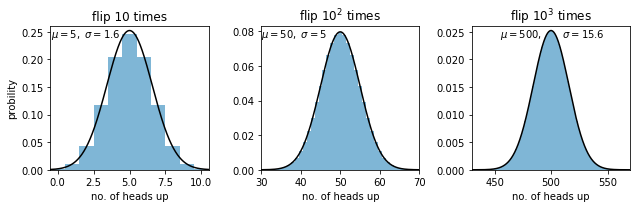
\includegraphics[width=.8\textwidth]{binomial.png} 
	\end{figure}
\end{frame}

\begin{frame}
    \frametitle{The Normal Distribution}
    \begin{itemize}[wide = 0pt]
        \item[$\square$]  The Normal distribution has the shape of a "bell curve" with parameters \textbf{\color{red}$\mu$} and \textbf{\color{red}$\sigma^2$} that determine the center and spread.
        \item[$\square$] Probability density function: $f(x)=\frac{1}{\sigma\sqrt{2\pi}}e^{\frac{(x-\mu)^2}{2\sigma^2}}$
    \end{itemize}
    \vspace{10pt}
    \begin{tikzpicture}
        \begin{axis}[
            no markers, 
            domain=0:6, 
            samples=100,
            ymin=0,
            axis lines*=left, 
            xlabel=$x$,
            every axis y label/.style={at=(current axis.above origin),anchor=south},
            every axis x label/.style={at=(current axis.right of origin),anchor=west},
            height=5cm, 
            width=12cm,
            xtick=\empty, 
            ytick=\empty,
            enlargelimits=false, 
            clip=false, 
            axis on top,
            grid = major,
            hide y axis
            ]

            \addplot [very thick,black] {gauss(x, 3, 1)};

            \pgfmathsetmacro\valueA{gauss(1,3,1)}
            \pgfmathsetmacro\valueB{gauss(2,3,1)}
            \pgfmathsetmacro\valueC{gauss(3,3,1)}

            \draw [gray] (axis cs:1,0) -- (axis cs:1,\valueA);
            \draw [gray] (axis cs:2,0) -- (axis cs:2,\valueB);
            \draw [gray] (axis cs:3,0) -- (axis cs:3,\valueC);
            \draw [stealth-stealth] (axis cs:2,\valueB) -- node[below] {$\sigma$} (axis cs:3,\valueB);

            \node[below] at (axis cs:1, 0)  {$\mu - 2\sigma$}; 
            \node[below] at (axis cs:2, 0)  {$\mu - \sigma$}; 
            \node[below] at (axis cs:3, 0)  {$\mu$}; 

        \end{axis}
    \end{tikzpicture}
\end{frame}

\begin{frame}
    \frametitle{The Normal Distribution (cont'd)}
    \begin{itemize}[wide = 0pt]
        \item[$\square$] Each different value of \textbf{$\mu$} and \textbf{$\sigma^2$} gives a different Normal distribution, denoted by \textbf{\color{red}$N(\mu,\sigma^2)$}.
    \end{itemize}
    \vspace{10pt}
    \begin{tikzpicture}
        \pgfmathsetlengthmacro\MajorTickLength{
        \pgfkeysvalueof{/pgfplots/major tick length} * 0.5
        }
        \begin{axis}[
            no markers, 
            domain=-6.2:6.2, 
            samples=100,
            ymin=-0.01,
            axis lines*=left, 
            xlabel=$x$,
            every axis y label/.style={at=(current axis.above origin),anchor=south},
            every axis x label/.style={at=(current axis.right of origin),anchor=west},
            height=5cm, 
            width=12cm,
            tick align=outside,
            xtick={-6,-4,-2,0,2,4,6}, 
            ytick=\empty,
            enlargelimits=false, 
            clip=false, 
            axis on top,
            hide y axis,
            major tick length=\MajorTickLength,
            every tick/.style={
            black, semithick},
            ]

            \addplot [thick,black] {gauss(x, 0, 1)};
            \addplot [thick,red] {gauss(x, -2, 1)};
            \addplot [thick,blue] {gauss(x, 0, 2)};
            \addplot [thick,green] {gauss(x, 2, 2)};
            
            \pgfmathsetmacro\valueA{gauss(0,0,1)}
            \pgfmathsetmacro\valueB{gauss(-3,-2,1)}
            \pgfmathsetmacro\valueC{gauss(0,0,2)}
            \pgfmathsetmacro\valueD{gauss(3,2,2)}
            
            \node[right] at (axis cs:0.2, \valueA)  {\small{$N(0,1)$}};
            \node[left,red] at (axis cs:-3,\valueB) {\small{$N(-2,1)$}};
            \node[above,blue] at (axis cs:0,\valueC) {\small{$N(0,2)$}};
            \node[right, green] at (axis cs:3.2,\valueD) {\small{$N(2,2)$}};
        \end{axis}
    \end{tikzpicture}
\end{frame}

\begin{frame}
    \frametitle{Properties of the Normal Distribution}
    \begin{tabular}{l c c c}
    \toprule
        Intervals & $(\mu-\sigma,\mu+\sigma)$ & $(\mu-2\sigma,\mu+2\sigma)$ & $(\mu-3\sigma,\mu+3\sigma)$ \\
        Probability & $68.27\%$ & $95.45\%$ & $99.73\%$ \\
        \midrule
        Intervals & $\mu\pm1.65\sigma$ & {\color{red}$\mu\pm1.96\sigma$} & $\mu\pm2.58\sigma$ \\
        Probability & $90\%$ & {\color{red}$95\%$} & $99\%$ \\
    \bottomrule
    \end{tabular} \\
    \vspace{10pt}
    \begin{tikzpicture}
        \begin{axis}[
            no markers, 
            domain=-3.2:3.2, 
            samples=100,
            ymin=0,
            axis lines*=left, 
            xlabel=$x$,
            every axis y label/.style={at=(current axis.above origin),anchor=south},
            every axis x label/.style={at=(current axis.right of origin),anchor=west},
            height=5cm, 
            width=12cm,
            xtick=\empty, 
            ytick=\empty,
            enlargelimits=false, 
            clip=false, 
            axis on top,
            hide y axis
            ]
            
            \addplot [black] {gauss(x, 0, 1)};
            
            \addplot [fill=black!5, draw=none, domain=-1:1] {gauss(x,0,1)} \closedcycle;
            \addplot [fill=blue!30, draw=none, domain=-1.65:-1] {gauss(x,0,1)} \closedcycle;
            \addplot [fill=blue!30, draw=none, domain=1:1.65] {gauss(x,0,1)} \closedcycle;
             \addplot [fill=red!30, draw=none, domain=-1.96:-1.65] {gauss(x,0,1)} \closedcycle;
            \addplot [fill=red!30, draw=none, domain=1.65:1.96] {gauss(x,0,1)} \closedcycle;
            \addplot [fill=black, draw=none, domain=-2:-1.96] {gauss(x,0,1)} \closedcycle;
            \addplot [fill=black, draw=none, domain=1.96:2] {gauss(x,0,1)} \closedcycle;
            
            \addplot [fill=green!30, draw=none, domain=-2.58:-2] {gauss(x,0,1)} \closedcycle;
            \addplot [fill=green!30, draw=none, domain=2:2.58] {gauss(x,0,1)} \closedcycle;
            
            \addplot [fill=yellow!30, draw=none, domain=-3:-2.58] {gauss(x,0,1)} \closedcycle;
            \addplot [fill=yellow!30, draw=none, domain=2.58:3] {gauss(x,0,1)} \closedcycle;

            \draw [black] (axis cs:0,0) -- (axis cs:0,-0.01);
            \node[below] at (axis cs:0,0)  {\small{$\mu$}};
            
            \draw [black] (axis cs:-1,0) -- (axis cs:-1,-0.01);
            \node[below] at (axis cs:-1,0)  {\scriptsize{$\mu-\sigma$}};
            \draw [black] (axis cs:-2,0) -- (axis cs:-2,-0.01);
            \node[below] at (axis cs:-2,0)  {\scriptsize{$\mu-2\sigma$}};
            \draw [black] (axis cs:-3,0) -- (axis cs:-3,-0.01);
            \node[below] at (axis cs:-3,0)  {\scriptsize{$\mu-3\sigma$}};
            
            \draw [black] (axis cs:1.65,0) -- (axis cs:1.65,-0.01);
            \node[below left] at (axis cs:1.65,0) {\scriptsize{$\mu+1.65\sigma$}};
            \draw [black] (axis cs:1.96,0) -- (axis cs:1.96,-0.01);
            \node[below] at (axis cs:1.96,0) {\scriptsize{$\mu+1.96\sigma$}};
            \draw [black] (axis cs:2.58,0) -- (axis cs:2.58,-0.01);
            \node[below right] at (axis cs:2.58,0) {\scriptsize{$\mu+2.58\sigma$}};
            
            \draw[gray] (axis cs:-3,0) -- (axis cs:-3,0.24) (axis cs:3,0) -- (axis cs:3,0.24);
            \draw[gray] (axis cs:-2.58,0) -- (axis cs:-2.58,0.24) (axis cs:2.58,0) -- (axis cs:2.58,0.24);
            \draw[gray] (axis cs:-2,0) -- (axis cs:-2,0.24) (axis cs:2,0) -- (axis cs:2,0.24);
            \draw[gray] (axis cs:-1.96,0) -- (axis cs:-1.96,0.24) (axis cs:1.96,0) -- (axis cs:1.96,0.24);
            \draw[gray] (axis cs:-1.65,0) -- (axis cs:-1.65,0.24) (axis cs:1.65,0) -- (axis cs:1.65,0.24);
            
            \draw[gray,stealth-stealth] (axis cs:-3,0.04) -- node[fill=black!5, text=black] {\tiny{$99.73\%$}} (axis cs:3,0.04);
            \draw[gray,stealth-stealth] (axis cs:-2.58,0.08) -- node[fill=black!5, text=black] {\tiny{$99\%$}} (axis cs:2.58,0.08);
            \draw[gray,stealth-stealth] (axis cs:-2,0.12) -- node[fill=black!5, text=black] {\tiny{$95.45\%$}} (axis cs:2,0.12);
            \draw[gray,stealth-stealth] (axis cs:-1.96,0.16) -- node[fill=black!5, text=black] {\tiny{$95\%$}} (axis cs:1.96,0.16);
            \draw[gray,stealth-stealth] (axis cs:-1.65,0.2) -- node[fill=black!5, text=black] {\tiny{$90\%$}} (axis cs:1.65,0.2);
            \draw[gray,stealth-stealth] (axis cs:-1,0.24) -- node[fill=black!5, text=black] {\tiny{$68.27\%$}} (axis cs:1,0.24);
        \end{axis}
    \end{tikzpicture}
\end{frame}

\begin{frame}
    \frametitle{Standardization}
    \begin{itemize}[wide = 0pt]
        \item[$\square$] If $N(0,1)$, it is called \textbf{\color{red}Standard Normal distribution}
        \item[$\square$] Any non-standard Normal distribution can be transformed into the standard one. This process is called \textbf{standardization}
        \item[$\square$] Why standardization: 
        \item[\ \ ] $P(x)=\int_{-\infty}^x\frac{1}{\sigma\sqrt{2\pi}}e^{\frac{(x-\mu)^2}{2\sigma^2}}dx$ $\rightarrow$ $P(x)=\int_{-\infty}^x\frac{1}{\sqrt{2\pi}}e^{\frac{x^2}{2}}dx$ 
        \item[$\square$] \textbf{Linear transformation} is used to convert a non-standard Normal distribution into the standard one
        \item[$\square$] If $X \sim N(\mu, \sigma^2)$, we want $Z \sim N(0, 1)$, then we use the following equation:
    \end{itemize}
    \begin{equation*}
        \color{red} Z=\frac{X-\mu}{\sigma}
    \end{equation*}
    \vspace*{\fill}
\end{frame}

\begin{frame}
    \frametitle{Practice 1}
    \begin{itemize}[wide = 0pt]
        \item[$\square$] Fill in the blanks
    \end{itemize}
    \begin{tabular}{l c c c c c c}
		\toprule
        \multicolumn{7}{c}{\textbf{$X \sim N(0,1)$}}  \\
        \midrule
			 Intervals & $(-1, 1)$ & & & $(-2,2)$ & & $(-3,3)$ \\
			 Probability & & $90\%$ & $95\%$ & & $99\%$ & \\
        \bottomrule
	\end{tabular}
	\vspace{20pt}
	\begin{itemize}[wide = 0pt]
        \item[$\square$] An array $\textbf{X}=[0, 1, 2, 3, 4, 5]$ follows the Normal distribution $N(7,25)$. Please convert this array and let it follow the Standard Normal distribution.
    \end{itemize}
    \vspace{\fill}
\end{frame}

\begin{frame}
    \frametitle{Solution 1}
    \begin{itemize}[wide = 0pt]
        \item[$\square$] $X \sim N(7,25)$ gives $\mu=7$, $\sigma=5$
        \vspace{5pt}
        \item[$\square$] and $\textbf{Z}=(\textbf{X}-\mu)/\sigma$
        \vspace{5pt}
        \item[$\square$] Hence, $\textbf{Z}=[-1.4, -1.2, -1.0, -0.8, -0.6, -.4]$
    \end{itemize} 
    \vspace{\fill}
\end{frame}

\begin{frame}
    \frametitle{Log Transformation for Skewed Distributions}
    \begin{itemize}[wide = 0pt]
        \item[$\square$] A distribution that is not symmetric but exhibit skewness with heavy right tail
        \item[$\square$] When appropriate the Log transformation has good statistical properties
        \item[$\square$] X is log-normal if log(X) is normally distributed and this property is key to transform your data back to its original scale
    \end{itemize}
    \begin{figure}
    \centering
    \begin{subfigure}{0.5\textwidth}
        \centering
        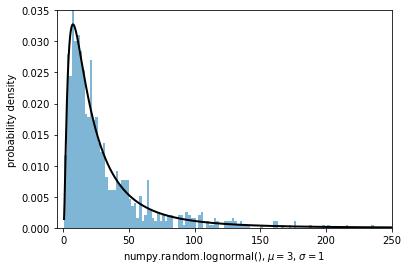
\includegraphics[width=.9\textwidth]{log1.png}
        % \caption{Lorem ipsum}
    \end{subfigure}%
    \begin{subfigure}{0.5\textwidth}
        \centering
        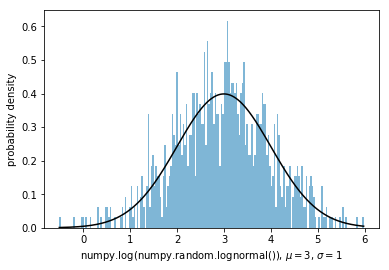
\includegraphics[width=.9\textwidth]{log2.png}
        % \caption{}
    \end{subfigure}
    % \caption{Caption place holder}
    \end{figure}
\end{frame}

\begin{frame}
    \frametitle{Sampling}
    \vspace{-8pt}
    \begin{itemize}[wide = 0pt]
        \item[$\square$] Statistical inference: using observed data to estimate characteristics of the whole population
        \begin{itemize}
            \item[--] Assumed that the observed data is sampled from population
            \item[--] Characteristics: mean, variance, correlation, etc ...
        \end{itemize}
        \item[$\square$] Factor that influences our ability to make inference from a sample to a population:
        \begin{itemize}
            \item[--] \textbf{Bias}: sample is not a representative of the whole population
        \end{itemize}
        \item[$\square$] Methods to avoid bias:
        \begin{itemize}
            \item[--] Random sampling: each element in the population has an equal probability of selection
            \item[--] Stratified sampling: random selection in each strata
            \item[--] Systematic sampling, cluster sampling, etc ...
        \end{itemize}
    \end{itemize}
    \vspace*{\fill}
\end{frame}

\begin{frame}
    \frametitle{Sampling Variability}
    \begin{itemize}[wide = 0pt]
        \item[$\square$] Example: Random sampling from Lognormal distribution $lnX\sim N(0,1)$, where $f(x)=\frac{1}{x\sigma\sqrt{2\pi}}exp(\frac{-(lnx-\mu)^2}{2\sigma^2})$
        \item[$\square$] 5 trials, 50 samples per trial. Each trial gives a different $\overline{lnX}$ and $s$
    \end{itemize} 
    \vspace{5pt}
    \begin{columns}[T]
		\column{0.0325\textwidth}
		\column{0.2675\textwidth}
		    \centering
		    \begin{tabular}{c c c}
		    \toprule
		       & $\overline{lnX}$ & $s$ \\
		    \hline
		      \small{1} & \small{-0.361} & \small{1.065} \\ 
		      \small{2} & \small{0.205} & \small{0.965} \\
		      \small{3} & \small{-0.138} & \small{0.914} \\
		      \small{4} & \small{-0.100} & \small{0.983} \\
		      \small{5} & \small{0.114} & \small{0.996} \\
		    \bottomrule
		    \end{tabular}
		\column{0.05\textwidth}
		\column{0.6375\textwidth}
			\centering
			\vspace{10pt}
			\begin{tikzpicture}[scale=0.65]
            \begin{axis}[
                no markers, 
                domain=0:3, 
                samples=100,
                ymin=-0.01,
                axis lines*=left, 
                every axis y label/.style={at=(current axis.above origin),anchor=south},
                every axis x label/.style={at=(current axis.right of origin),anchor=west},
                height=5cm, 
                width=12cm,
                tick align=outside,
                xtick=\empty,
                ytick=\empty,
                enlargelimits=false, 
                clip=false, 
                axis on top,
                hide y axis
                ]
                \addplot [very thick,black] {lognormal(x,0,1)};
                \pgfmathsetmacro\valueA{lognormal(1,0,1)}
                \node[right] at (axis cs:1.1,\valueA)  {\textbf{$f(x)$}};
            \end{axis}
        \end{tikzpicture}
		\column{0.0125\textwidth}
	\end{columns}
	\vspace*{\fill}
\end{frame}

\begin{frame}
    \frametitle{Distribution of the Sample Mean}
    \begin{itemize}[wide = 0pt]
        \item[$\square$] What is the distribution of sample mean $\overline{X}$, or $\overline{lnX}$ in the previous example?
        \vspace{8pt}
        \item[$\square$] \textbf{\color{red}Central Limit Theorem}: If a random sample $X$ with n observations is drawn from a population with finite mean $\mu$ and variance $\sigma^2$, then, when n is {\color{red}sufficiently large} ($n > 30$), the sample mean $\overline{X}$ can be approximated by {\color{red}$\overline{X}\sim N(\mu,\sigma^2/n)$}
        \begin{itemize}
            \item[--] Sufficiently large: typically $n > 30$
            \item[--] Distribution of X is not necessarily Normal
            \item[--] Allow us use sample mean $\overline{X}$ to make statistical inferences about the population mean $\mu$
        \end{itemize}
    \end{itemize}
    \vspace*{\fill}
\end{frame}

\begin{frame}
    \frametitle{Distribution of the Sample Mean (cont'd)}
    \begin{itemize}[wide = 0pt]
        \item[$\square$] Example: $lnX\sim N(0,1)$, 10000 trials with 50 samples per trial. Plot the sample mean $\overline{ln\textbf{X}}$
        \item[$\square$] According to Central Limit Theorem, we derive that the sample mean $\overline{X}$ can be approximated by $\overline{X}\sim N(0, 1/50)$
    \end{itemize}
    \begin{figure}
        \centering
		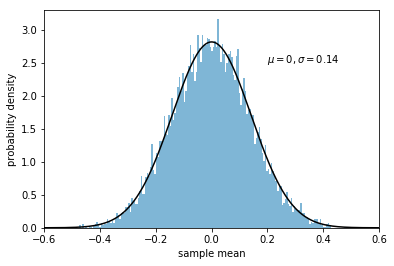
\includegraphics[width=.6\textwidth]{lognormal.png}
	\end{figure}
	\vspace*{\fill}
\end{frame}

\begin{frame}
    \frametitle{What if $n \leq 30$? Student's t-Distribution}
    \begin{tikzpicture}
        \begin{axis}[
            no markers, 
            domain=-5:5, 
            samples=100,
            ymin=-0.01,
            axis lines*=left, 
            xlabel=$x$,
            every axis y label/.style={at=(current axis.above origin),anchor=south},
            every axis x label/.style={at=(current axis.right of origin),anchor=west},
            height=6cm, 
            width=12cm,
            xtick=\empty, 
            ytick=\empty,
            enlargelimits=false, 
            clip=false, 
            axis on top,
            grid = major,
            hide y axis,
            legend style={font=\small},
            legend entries={$df = 1\ $,
                          $df = 2\ $,
                          $df = 5\ $,
                          $df = 10$,
                          $df = \infty$
                          }
            ]

            \addplot [thick,gray] {student(x, 1)};
            \addplot [thick,orange] {student(x, 2)};
            \addplot [thick,red] {student(x, 5)};
            \addplot [thick,blue] {student(x, 10)};
            \addplot [thick,black] {gauss(x, 0, 1)};

        \end{axis}
    \end{tikzpicture}
\end{frame}

\begin{frame}
    \frametitle{Student's t-Distribution}
    \begin{itemize}[wide = 0pt]
        \item[$\square$] When {\color{red}$n\leq30$} and {\color{red}$\sigma$ unknown}, use \textbf{Student's t-distribution} instead of Normal distribution
        \vspace{5pt}
        \item[$\square$] Closely related to standard Normal distribution
        \begin{itemize}
            \item[--] Continuous probability distribution
            \item[--] Heavier tails
            \item[--] 1 additional parameter: degree of freedom (df)
        \end{itemize}
        \vspace{5pt}
        \item[$\square$] For univariate t-distribution, $df = n - 1$
    \end{itemize}
    \vspace*{\fill}
\end{frame}

\begin{frame}
    \frametitle{Sampling Variability and Standard Error}
    \begin{itemize}[wide = 0pt]
        \item[$\square$] \textbf{\color{red}Standard Error} (SE) of the mean is the standard deviation (SD) of the sample mean, which quantifies the accuracy of the sample mean $\overline{X}$ as an estimate of the population mean $\mu$
        \vspace{8pt}
        \item[$\square$] Standard error calculation
        \begin{itemize}
            \item[--] If $\sigma$ is known, SE is calculated by $SE = \sigma/\sqrt{n}$
            \item[--] If $\sigma$ is unknown, SE is estimated by $SE \approx s/\sqrt{n}$
            \item[--] Where $\sigma$ is the population standard deviation, $s$ is the sample standard deviation, and $n$ is the sampling size
        \end{itemize}
    \end{itemize}
    \vspace*{\fill}
\end{frame}

\begin{frame}
    \frametitle{Standard Deviation vs. Standard Error}
    \begin{itemize}[wide = 0pt]
        \item[$\square$] Standard error: quantifies the typical error or difference between the sample mean $\overline{X}$ and the theoretical mean $\mu$ in the population from which the sample was drawn
        \begin{equation*}
            SE = \frac{\sigma}{\sqrt{n}}
        \end{equation*}
        \item[$\square$] Standard deviation of a sample of observations measures how a typical observation in the sample deviates from the sample mean
        \begin{equation*}
            SD = \sqrt{\frac{1}{n-1}\sum_{i=1}^n(x_i-\mu)^2}
        \end{equation*}
    \end{itemize}
\end{frame}

\begin{frame}
    \frametitle{Practice 2}
    \begin{itemize}[wide = 0pt]
        \item[$\square$] You are investigating the Body Mass Index for people with different diet, calculate standard deviation and standard error for the two diet groups
    \end{itemize}
    \vspace{15pt}
    \centering
    \begin{tabular}{p{0.04\linewidth} p{0.04\linewidth} p{0.04\linewidth} p{0.04\linewidth} p{0.04\linewidth} p{0.04\linewidth} p{0.04\linewidth} p{0.04\linewidth} p{0.04\linewidth} p{0.04\linewidth} p{0.04\linewidth} p{0.04\linewidth}}
    \toprule
        \multicolumn{12}{c}{Diet 1: low consumption of fruit/veg}  \\
        & \small{24.1} & \small{23.5} & \small{18.5} & \small{16.7} & \small{26.3} & \small{28.5} & \small{25.2} & \small{23.4} & \small{22.5} & \small{29.9} & \\
        \midrule
        \multicolumn{12}{c}{Diet 2: high consumption of fruit/veg} \\
        \small{22.1} & \small{20.5} & \small{18.5} & \small{16.9} & \small{24.1} & \small{26.0} & \small{22.2} & \small{28.4} & \small{21.5} & \small{31.9} & \small{23.0} & \small{17.2} \\
        \bottomrule
    \end{tabular}
    \vspace*{\fill}
\end{frame}

\begin{frame}
    \frametitle{Solution 2}
    \begin{itemize}[wide = 0pt]
        \item[$\square$] $n_{d1} = 10$, $n_{d2} = 12$ 
        \vspace{5pt}
        \item[$\square$] $\mu_{d1}=23.86$, $\mu_{d2}=22.69$
        \vspace{5pt}
        \item[$\square$] $SD_{d1} = 4.06$, $SD_{d2} = 4.47$
        \vspace{5pt}
        \item[$\square$] $SE_{d1} = 1.28$, $SE_{d2} = 1.29$
    \end{itemize} 
    
\end{frame}

\begin{frame}
    \frametitle{Confidence Intervals}
    \begin{itemize}[wide = 0pt]
        \item[$\square$] \textbf{\color{red}Confidence interval} (CI) quantifies the level of confidence that the parameter lies in the interval
        \begin{itemize}
            \item[--] e.g. level of confidence that CI contains the true value of the population mean $\mu$
        \end{itemize}
        \vspace{5pt}
        \item[$\square$] Factors required to construct a confidence interval for the true value of the population mean
        \begin{itemize}
            \item[--] {\color{red}Sample mean} $\overline{X}$
            \item[--] {\color{red}Standard error} of the mean $\sigma/\sqrt{n}$
            \item[--] {\color{red}Sample mean distribution}, e.g. Normal distribution
            \item[--] {\color{red}Level of confidence}, e.g. $95\%$
        \end{itemize}
    \end{itemize}
    \vspace*{\fill}
\end{frame}

\begin{frame}
    \frametitle{Confidence Intervals (cont'd)}
    \begin{itemize}[wide = 0pt]
        \item[$\square$] Constructing a $95\%$ confidence interval, when $n>30$
        \begin{itemize}
            \item[--] If \small{$X\sim N(\mu, \sigma^2)$}, \small{$\overline{X}\sim N(\mu, \sigma^2/n)$}
            \item[--] Standardization $\overline{X}$ gives:
            \begin{equation}
                {\color{red}Z=\frac{\overline{X}-\mu}{\sigma/\sqrt{n}}\sim N(0,1)}
                \label{eq:standardization_ci}
            \end{equation}
            \item[--] $95\%$ confidence interval refers to \small{$P(-1.96<Z<1.96)=0.95$}
            \item[--] Replace $Z$ by equation (\ref{eq:standardization_ci}) gives:
            \begin{equation*}
                P(\overline{X}-1.96\frac{\sigma}{\sqrt{n}}<\mu<\overline{X}+1.96\frac{\sigma}{\sqrt{n}})=0.95
            \end{equation*}
        \end{itemize}
    \end{itemize}
    \vspace*{\fill}
\end{frame}

\begin{frame}
    \frametitle{Confidence Intervals (cont'd)}
    \begin{itemize}[wide = 0pt]
        \item[$\square$] Constructing a $95\%$ confidence interval, when $n>30$
        \vspace{5pt}
        \begin{itemize}
            \item[--] Therefore, $95\%$ confidence interval for the true population mean $\mu$ is
            \begin{equation*}
                (\overline{X}-1.96\frac{\sigma}{\sqrt{n}}, \overline{X}+1.96\frac{\sigma}{\sqrt{n}})
            \end{equation*}
            \item[--] Out of 100 samples, if we obtain a CI as above, 95 will contain the true but unknown population mean $\mu$
            \item[--] Or, we are $95\%$ sure that the true but unknown population mean $\mu$ lies on CI obtained from a sample mean $\overline{X}$
            \end{itemize}
    \end{itemize}
    \vspace*{\fill}
\end{frame}

\begin{frame}
    \frametitle{Confidence Intervals: Example}
    \vspace{-5pt}
    \begin{itemize}[wide = 0pt]
        \item[$\square$] Investigating BMI for women living in rural areas of Bangladesh
    \end{itemize}
    \centering
    \begin{tabular}{p{0.038\linewidth} p{0.038\linewidth} p{0.038\linewidth} p{0.038\linewidth} p{0.038\linewidth} p{0.038\linewidth} p{0.038\linewidth} p{0.038\linewidth} p{0.038\linewidth} p{0.038\linewidth} p{0.038\linewidth} p{0.038\linewidth} p{0.038\linewidth}}
    \toprule
        \small{18.1} & \small{21.6} & \small{19.5} & \small{21.0} & \small{26.8} & \small{19.4} & \small{21.0} & \small{23.8} & \small{19.1} & \small{19.5} & \small{21.7} & \small{22.9} & \small{22.9} \\
        
        \small{18.0} & \small{18.1} & \small{17.0} & \small{17.6} & \small{15.6} & \small{21.3} & \small{19.8} & \small{22.3} & \small{20.8} & \small{18.1} & \small{22.1} & \small{23.6} & \small{19.2} \\
        
        \small{18.6} & \small{25.6} & \small{21.6} & \small{17.7} & \small{20.9} & \small{20.8} & \small{23.5} & \small{15.9} & \small{20.0} & \small{18.6} & \small{23.2} & \small{22.2} & \small{21.3} \\
        
        \small{13.5} & \small{16.8} & \small{19.4} & \small{21.2} & \small{18.8} & \small{23.2} & \small{18.0} & \small{17.5} & \small{18.0} & \small{19.5} & \small{20.6} \\
    \bottomrule
    \end{tabular}
    \begin{columns}[T]
		\column{0.0125\textwidth}
		\column{0.4875\textwidth}
			\centering
            \begin{figure}
                \centering
                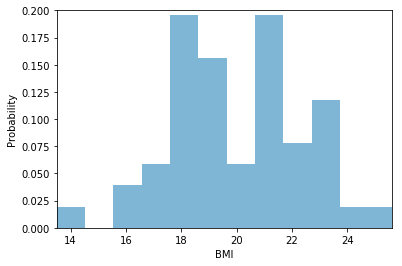
\includegraphics[width=.95\textwidth]{bmi_ci.png}
            \end{figure}
		\column{0.4875\textwidth}
		\vspace{15pt}
			\centering
			\begin{tabular}{l l}
			\toprule
			    \multicolumn{2}{c}{Summary Statistics} \\
			    Mean & 20.14 \\
			    Standard Deviation & 2.60 \\
			    Sample Size & 50 \\
			    Standard Error & 0.37 \\
			\bottomrule
			\end{tabular}
		\column{0.0125\textwidth}
	\end{columns}
% 	\vspace*{\fill}
\end{frame}

\begin{frame}
    \frametitle{Confidence Intervals: Example (cont'd)}
    \begin{itemize}[wide = 0pt]
        \item[$\square$] Sample mean $\overline{X}=20.14$, however it is probably not exactly equal to the population mean $\mu$
        \item[$\square$] We need to use sample mean to calculate a confidence interval of likely values for the population mean $\mu$
        \item[$\square$] Assume:
        \begin{itemize}
            \item[--] Each observation is independently and randomly sampled from the population with unknown mean $\mu$
            \item[--] Population standard deviation $\sigma$ is equal to the sample standard deviation $s$, i.e. $\sigma=s$
        \end{itemize}
        \item[$\square$] Then, $\overline{X}\sim N(\mu, \sigma^2/n)$
    \end{itemize}
    \vspace*{\fill}
\end{frame}

\begin{frame}
    \frametitle{Confidence Intervals: Example (cont'd)}
    \begin{itemize}[wide = 0pt]
        \item[$\square$] A $95\%$ confidence interval is given by 
        \begin{equation*}
            (\overline{X}-1.96\frac{\sigma}{\sqrt{n}}, \overline{X}+1.96\frac{\sigma}{\sqrt{n}})
        \end{equation*}
        \item[$\square$] Replacing $\sigma$ and $n$ from sample statistics, we have
        \begin{equation*}
            (\square \square.\square \square, \square \square.\square \square)(practice \ 3)
        \end{equation*}
        \item[$\square$] We are $95\%$ sure that the true population mean $\mu$ lies within this confidence interval
    \end{itemize}
    \vspace*{\fill}
\end{frame}

\begin{frame}
    \frametitle{Solution 3}
    \begin{itemize}[wide = 0pt]
        \item[$\square$] $(\overline{X}-1.96SE, \overline{X}+1.96SE)$
        \vspace{5pt}
        \item[$\square$] $\overline{X}=20.14$, $SE=0.37$
        \vspace{5pt}
        \item[$\square$] $(19.41, 20.87)$
    \end{itemize} 
    
\end{frame}

\begin{frame}
    \frametitle{Critical Value}
    \begin{itemize}[wide = 0pt]
        \item[$\square$] A $95\%$ confidence interval $(\overline{X}-1.96\sigma/\sqrt{n}, \overline{X}+1.96\sigma/\sqrt{n})$
            \begin{itemize}
                \item[--] $95\%$: \textbf{confidence level}
                \item[--] $1.96$: \textbf{critical value} $(Z)$
            \end{itemize}
        \item[$\square$] General formula for a $100C\%$ confidence interval for population mean $\mu$ when $\sigma$ is known
        \begin{equation*}
            {\color{red}(\overline{X}-Z\frac{\sigma}{\sqrt{n}},\  \overline{X}+Z\frac{\sigma}{\sqrt{n}})}
        \end{equation*}
        \begin{itemize}
            \item[--] where $Z^*$ is the value from a standard Normal table that gives you a tail probability of $(1-C)/2$
            \item[--] A $95\%$ confidence interval where $C=0.95$ gives a tail probability of $0.025$
        \end{itemize}
    \end{itemize}
    \vspace*{\fill}
\end{frame}

\begin{frame}
    \frametitle{Critical Value: Example}
    \centering
    \begin{tabular}{l c c c}
    \toprule
        Confidence Level & $90\%$ & $95\%$ & $99\%$ \\
        Critical Value $Z$ & 1.65 & 1.96 & 2.58 \\
    \bottomrule
    \end{tabular} \\
    \vspace{15pt}
    \begin{tikzpicture}
        \begin{axis}[
            no markers, 
            domain=-3.2:3.2, 
            samples=100,
            ymin=0,
            axis lines*=left, 
            xlabel=$Z$,
            every axis y label/.style={at=(current axis.above origin),anchor=south},
            every axis x label/.style={at=(current axis.right of origin),anchor=west},
            height=5cm, 
            width=12cm,
            xtick=\empty, 
            ytick=\empty,
            enlargelimits=false, 
            clip=false, 
            axis on top,
            hide y axis
            ]
            
            \addplot [black] {gauss(x, 0, 1)};
            
            \addplot [fill=black!5, draw=none, domain=-1.65:1.65] {gauss(x,0,1)} \closedcycle;
            \addplot [fill=blue!30, draw=none, domain=-1.96:-1.65] {gauss(x,0,1)} \closedcycle;
            \addplot [fill=blue!30, draw=none, domain=1.65:1.96] {gauss(x,0,1)} \closedcycle;
            \addplot [fill=red!30, draw=none, domain=-2.58:-1.96] {gauss(x,0,1)} \closedcycle;
            \addplot [fill=red!30, draw=none, domain=1.96:2.58] {gauss(x,0,1)} \closedcycle;
            \addplot [fill=red!30!blue!30, draw=none, domain=-3.2:-2.58] {gauss(x,0,1)} \closedcycle;
            \addplot [fill=red!30!blue!30, draw=none, domain=2.58:3.2] {gauss(x,0,1)} \closedcycle;

            \draw [black] (axis cs:0,0) -- (axis cs:0,-0.01);
            \node[below] at (axis cs:0,0)  {\scriptsize{0}};
            
            \draw [black] (axis cs:-1.65,0) -- (axis cs:-1.65,-0.01);
            \node[below right] at (axis cs:-1.65,0) {\scriptsize{-1.65}};
            \draw [black] (axis cs:-1.96,0) -- (axis cs:-1.96,-0.01);
            \node[below] at (axis cs:-1.96,0) {\scriptsize{-1.96}};
            \draw [black] (axis cs:-2.58,0) -- (axis cs:-2.58,-0.01);
            \node[below] at (axis cs:-2.58,0) {\scriptsize{-2.58}};
            
            \draw [black] (axis cs:1.65,0) -- (axis cs:1.65,-0.01);
            \node[below left] at (axis cs:1.65,0) {\scriptsize{1.65}};
            \draw [black] (axis cs:1.96,0) -- (axis cs:1.96,-0.01);
            \node[below] at (axis cs:1.96,0) {\scriptsize{1.96}};
            \draw [black] (axis cs:2.58,0) -- (axis cs:2.58,-0.01);
            \node[below] at (axis cs:2.58,0) {\scriptsize{2.58}};
            

            \draw[gray] (axis cs:-2.58,0) -- (axis cs:-2.58,0.24) (axis cs:2.58,0) -- (axis cs:2.58,0.24);
            \draw[gray] (axis cs:-1.96,0) -- (axis cs:-1.96,0.24) (axis cs:1.96,0) -- (axis cs:1.96,0.24);
            \draw[gray] (axis cs:-1.65,0) -- (axis cs:-1.65,0.24) (axis cs:1.65,0) -- (axis cs:1.65,0.24);
            
            \draw[gray,stealth-stealth] (axis cs:-2.58,0.06) -- node[fill=black!5, text=black] {\tiny{$99\%$}} (axis cs:2.58,0.06);
            \draw[gray,stealth-stealth] (axis cs:-1.96,0.12) -- node[fill=black!5, text=black] {\tiny{$95\%$}} (axis cs:1.96,0.12);
            \draw[gray,stealth-stealth] (axis cs:-1.65,0.18) -- node[fill=black!5, text=black] {\tiny{$90\%$}} (axis cs:1.65,0.18);
            
            \node[above] at (axis cs:0,0.24)  {\scriptsize{$Area=C$}};
        \end{axis}
    \end{tikzpicture}
\end{frame}

\begin{frame}
    \frametitle{Confidence Intervals: What if $n\leq30$?}
    \centering
    \begin{tabular}{l c c}
    \toprule
          & $n>30$ & $n\leq30$ \\
         Known $\sigma$ & $Z\sim N(0,1)$ & $Z\sim N(0,1)$ \\
         Unknown $\sigma$ & $Z\sim N(0,1)$ (approx.) & {\color{red}$T\sim t_{df}$} \\
    \bottomrule
    \end{tabular}
    \vspace{5pt}
    \begin{itemize}[wide = 0pt]
        \item[$\square$] For $Z\sim N(0,1)$, we have
        \begin{equation*}
            Z=\frac{\overline{X}-\mu}{\sigma/\sqrt{n}}
        \end{equation*}
        \item[$\square$] For $T\sim t_{df}$, where $t_{df}$ is a Student t-distribution, we have
        \begin{equation*}
            \color{red}T=\frac{\overline{X}-\mu}{s/\sqrt{n}}
        \end{equation*}
    \end{itemize}
\end{frame}

\begin{frame}
    \frametitle{Confidence Intervals: Student's t-Distribution}
    \begin{itemize}[wide = 0pt]
        \item[$\square$] If $\sigma$ is unknown and sample size is large $(n>30)$, $t_{df}$ where $df=n-1$ approximates the standard Normal distribution
        \item[$\square$] General formula for a $100C\%$ confidence interval for population mean $\mu$ when $\sigma$ is unknown and $n\leq30$:
        \begin{equation*}
            {\color{red}(\overline{X}-Ts/{\sqrt{n}},\ \overline{X}+Ts/{\sqrt{n}})}
        \end{equation*}
        \item[$\square$] Example: $95\%$ confidence interval for 9 observations $(n=9)$ with known and unknown $\sigma$
    \end{itemize}
    \vspace{5pt}
    \centering
    \begin{tabular}{c c}
    \toprule
         Known $\sigma$ & Unknown $\sigma$ \\
         $(\overline{X}-{\color{red}1.96}\sigma/3,\ \overline{X}+{\color{red}1.96}\sigma/3)$ & $(\overline{X}-{\color{red}2.31}s/3,\ \overline{X}+{\color{red}2.31}s/3)$\\
    \bottomrule
    \end{tabular}
    \vspace*{\fill}
\end{frame}

\begin{frame}
    \frametitle{$95\%$ Confidence Interval Tail Areas}
    \begin{figure}
        \centering
        \begin{subfigure}[b]{0.475\textwidth}
            \centering
            \begin{tikzpicture}[scale=0.5]
            \pgfmathsetlengthmacro\MajorTickLength{
            \pgfkeysvalueof{/pgfplots/major tick length}}
                \begin{axis}[
                    no markers, 
                    domain=-4.2:4.2, 
                    samples=100,
                    ymin=0,
                    ymax=0.45,
                    axis lines*=left, 
                    height=6cm, 
                    width=11cm,
                    tick align=outside,
                    xtick={-4,-2,0,2,4}, 
                    ytick={0,0.2,0.4},
                    enlargelimits=false,
                    y axis line style = {-stealth},
                    clip=false, 
                    axis on top,
                    % hide y axis,
                    major tick length=\MajorTickLength,
                    every tick/.style={black, semithick},
                    legend entries={$df=3$}
                    ]
                    
                    \addplot [black] {student(x, 3)};
                    
                    \addplot [fill=black!5, draw=none, domain=-3.18:3.18] {student(x, 3)} \closedcycle;
                    \addplot [fill=blue!80, draw=none, domain=-4.2:-3.18] {student(x, 3)} \closedcycle;
                    \addplot [fill=blue!80, draw=none, domain=3.18:4.2] {student(x, 3)} \closedcycle;
                    
                    \node[above] at (axis cs:-3.18,0.2) {-3.18};
                    \node[above] at (axis cs:3.18,0.2) {3.18};
    
                    \draw[gray] (axis cs:-3.18,0) -- (axis cs:-3.18,0.2) (axis cs:3.18,0) -- (axis cs:3.18,0.2);
                \end{axis}
            \end{tikzpicture}
        \end{subfigure}
        \hfill
        \begin{subfigure}[b]{0.475\textwidth}  
            \centering 
            \begin{tikzpicture}[scale=0.5]
            \pgfmathsetlengthmacro\MajorTickLength{
            \pgfkeysvalueof{/pgfplots/major tick length}}
                \begin{axis}[
                    no markers, 
                    domain=-4.2:4.2, 
                    samples=100,
                    ymin=0,
                    ymax=0.45,
                    axis lines*=left, 
                    height=6cm, 
                    width=11cm,
                    tick align=outside,
                    xtick={-4,-2,0,2,4}, 
                    ytick={0,0.2,0.4},
                    enlargelimits=false,
                    y axis line style = {-stealth},
                    clip=false, 
                    axis on top,
                    % hide y axis,
                    major tick length=\MajorTickLength,
                    every tick/.style={black, semithick},
                    legend entries={$df=5$}
                    ]
                    
                    \addplot [black] {student(x, 5)};
                    
                    \addplot [fill=black!5, draw=none, domain=-2.57:2.57] {student(x, 5)} \closedcycle;
                    \addplot [fill=blue!80, draw=none, domain=-4.2:-2.57] {student(x, 5)} \closedcycle;
                    \addplot [fill=blue!80, draw=none, domain=2.57:4.2] {student(x, 5)} \closedcycle;
                    
                    \node[above] at (axis cs:-2.57,0.2) {-2.57};
                    \node[above] at (axis cs:2.57,0.2) {2.57};
    
                    \draw[gray] (axis cs:-2.57,0) -- (axis cs:-2.57,0.2) (axis cs:2.57,0) -- (axis cs:2.57,0.2);
                \end{axis}
            \end{tikzpicture}
        \end{subfigure}
        \vskip\baselineskip
        \begin{subfigure}[b]{0.475\textwidth}   
            \centering 
            \begin{tikzpicture}[scale=0.5]
            \pgfmathsetlengthmacro\MajorTickLength{
            \pgfkeysvalueof{/pgfplots/major tick length}}
                \begin{axis}[
                    no markers, 
                    domain=-4.2:4.2, 
                    samples=100,
                    ymin=0,
                    ymax=0.45,
                    axis lines*=left, 
                    height=6cm, 
                    width=11cm,
                    tick align=outside,
                    xtick={-4,-2,0,2,4}, 
                    ytick={0,0.2,0.4},
                    enlargelimits=false,
                    y axis line style = {-stealth},
                    clip=false, 
                    axis on top,
                    % hide y axis,
                    major tick length=\MajorTickLength,
                    every tick/.style={black, semithick},
                    legend entries={$df=30$}
                    ]
                    
                    \addplot [black] {student(x, 30)};
                    
                    \addplot [fill=black!5, draw=none, domain=-2.04:2.04] {student(x, 30)} \closedcycle;
                    \addplot [fill=blue!80, draw=none, domain=-4.2:-2.04] {student(x, 30)} \closedcycle;
                    \addplot [fill=blue!80, draw=none, domain=2.04:4.2] {student(x, 30)} \closedcycle;
                    
                    \node[above] at (axis cs:-2.04,0.2) {-2.04};
                    \node[above] at (axis cs:2.04,0.2) {2.04};
    
                    \draw[gray] (axis cs:-2.04,0) -- (axis cs:-2.04,0.2) (axis cs:2.04,0) -- (axis cs:2.04,0.2);
                \end{axis}
            \end{tikzpicture}
        \end{subfigure}
        \quad
        \begin{subfigure}[b]{0.475\textwidth}   
            \centering 
            \begin{tikzpicture}[scale=0.5]
            \pgfmathsetlengthmacro\MajorTickLength{
            \pgfkeysvalueof{/pgfplots/major tick length}}
                \begin{axis}[
                    no markers, 
                    domain=-4.2:4.2, 
                    samples=100,
                    ymin=0,
                    ymax=0.45,
                    axis lines*=left, 
                    height=6cm, 
                    width=11cm,
                    tick align=outside,
                    xtick={-4,-2,0,2,4}, 
                    ytick={0,0.2,0.4},
                    enlargelimits=false,
                    y axis line style = {-stealth},
                    clip=false, 
                    axis on top,
                    % hide y axis,
                    major tick length=\MajorTickLength,
                    every tick/.style={black, semithick},
                    legend entries={$df=\infty$}
                    ]
                    
                    \addplot [black] {gauss(x, 0, 1)};
                    
                    \addplot [fill=black!5, draw=none, domain=-1.96:1.96] {gauss(x, 0, 1)} \closedcycle;
                    \addplot [fill=blue!80, draw=none, domain=-4.2:-1.96] {gauss(x, 0, 1)} \closedcycle;
                    \addplot [fill=blue!80, draw=none, domain=1.96:4.2] {gauss(x, 0, 1)} \closedcycle;
                    
                    \node[above] at (axis cs:-1.96,0.2) {-1.96};
                    \node[above] at (axis cs:1.96,0.2) {1.96};
    
                    \draw[gray] (axis cs:-1.96,0) -- (axis cs:-1.96,0.2) (axis cs:1.96,0) -- (axis cs:1.96,0.2);
                \end{axis}
            \end{tikzpicture}
        \end{subfigure}
    \end{figure}
\end{frame}

\begin{frame}
    \frametitle{Confidence Intervals: Student's t-Distribution}
    \begin{itemize}[wide = 0pt]
        \item[$\square$] A confidence interval based on Student t-distribution will be {\color{red}wider} than the corresponding interval based on the Normal distribution
        \item[$\square$] \textbf{Intuition}
        \begin{itemize}
            \item[--] Sample standard deviation is likely to be poor estimate of population standard deviation $\sigma$, when sample size is small
            \item[--] Confidence interval using sample standard deviation $s$ should be wider than using $\sigma$
        \end{itemize}
        \item[$\square$] Student t-distribution with large sample size $(n>30)$ is approximately the standard Normal distribution, so confidence intervals will be about the same under both distributions
    \end{itemize}
    \vspace*{\fill}
\end{frame}

\begin{frame}
    \frametitle{Difference between Two Population Means: Example}
    \begin{itemize}[wide = 0pt]
        \item[$\square$] The birth weights of babies have been measured for a sample of mothers splitting into two categories: nonsmoking and heavy smoking
        \begin{itemize}
            \item[--] Two categories are measured independently from each other
            \item[--] Both come from Normal distributions
            \item[--] Same unknown variance $\sigma$
        \end{itemize}
        \item[$\square$] We want to know is there a significant difference in mean birth weights between the two categories
    \end{itemize}
    \vspace*{\fill}
\end{frame}

\begin{frame}
    \frametitle{Difference between Two Population Means: Example (cont'd)}
    \begin{itemize}[wide = 0pt]
        \item[$\square$] Summary of Data
    \end{itemize}
    \begin{tabular}{l c c c c c c c c c}
    \toprule
        Category & \multicolumn{4}{c}{\textbf{Non-smoking}} & & \multicolumn{4}{c}{\textbf{Heavy smoking}} \\
        \midrule
        \multirow{4}{*}{Weight (kg)} & \small{3.99} & \small{3.79} & \small{3.60} & \small{3.73} & & \small{3.18} & \small{2.84} & \small{2.90} & \small{3.27} \\
        & \small{3.21} & \small{3.60} & \small{4.08} & \small{3.61} & & \small{3.85} & \small{3.52} & \small{3.23} & \small{2.76} \\
        & \small{3.83} & \small{3.31} & \small{4.13} & \small{3.26} & & \small{3.60} & \small{3.75} & \small{3.59} & \small{3.63} \\
        & \small{3.54} & \small{3.51} & \small{2.71} & & & \small{2.38} & \small{2.34} & & \\
        \midrule
        Sample size & \multicolumn{4}{c}{\small{$n_1=15$}} & & \multicolumn{4}{c}{\small{$n_2=14$}} \\
        Mean &  \multicolumn{4}{c}{\small{$\overline{X}_1=3.59$}} & & \multicolumn{4}{c}{\small{$\overline{X}_2=3.20$}} \\
        Sample SD &  \multicolumn{4}{c}{\small{$s_1=0.37$}} & & \multicolumn{4}{c}{\small{$s_2=0.49$}} \\
        \bottomrule
    \end{tabular}
    \vspace*{\fill}
\end{frame}

\begin{frame}
    \frametitle{Difference between Two Population Means: Example (cont'd)}
    \begin{itemize}[wide = 0pt]
        \item[$\square$] The difference between the sample means
    \end{itemize}
    \begin{equation*}
        d_{\overline{X}}=\overline{X}_1 - \overline{X}_2=0.39
    \end{equation*}
    \begin{itemize}[wide = 0pt]
        \item[$\square$] The difference $d_{\overline{X}}$ arises by chance, or it is significant?
        \item[$\square$] Build the confidence interval for the difference between population means $d_{\mu}=\mu_1 - \mu_2$
        \begin{itemize}
            \item[--] $(d_{\overline{X}}-t_{df}s_E,\ d_{\overline{X}}+t_{df}s_E)$
            \item[--] If CI contains 0, $d_{\overline{X}}$ could arise by chance
            \item[--] Otherwise, it could be significant
        \end{itemize}
    \end{itemize}
    \vspace*{\fill}
\end{frame}

\begin{frame}
    \frametitle{Practice 4}
    \begin{itemize}[wide = 0pt]
        \item[$\square$] Build the confidence interval for $\mu$ at $95\%$ confidence level, given following equations derived from the Student's t-distribution:
        \begin{itemize}
            \item[--] Sample SE for difference of two sample means:
            \begin{equation*}
                s_E^2 = s_p^2(\frac{1}{n_1}+\frac{1}{n_2})
            \end{equation*}
            \item[--] Where
            \begin{equation*}
                s_p^2=\frac{(n_1-1)s_1^2+(n_2-1)s_2^2}{n_1+n_2-2}
            \end{equation*}
            \item[--] Critical value at $df=27$: $t_{df}=2.05$
        \end{itemize}
        \item[$\square$] What conclusion can we draw? [ans: $(0.06, 0.72)$]
    \end{itemize}
    \vspace*{\fill}
\end{frame}

\begin{frame}
    \frametitle{Hypothesis Testing}
    \vspace{-5pt}
    \begin{itemize}[wide = 0pt]
        \item[$\square$] Alternative method: other than constructing a confidence interval, we assume that there is no difference in mean birth weights between the two categories, i.e. $d_{\mu}=0$. Then we calculate under which condition the assumption does not hold
        \item[$\square$] The alternative method is called the \textbf{\color{red}hypothesis testing}
        \item[$\square$] Hypothesis
        \begin{itemize}
            \item[--] \textbf{\color{red}Null hypothesis} $(H_0)$: A default position that there is no effect or change between two measured phenomena, any differences are due to chance. e.g. $d_{\mu}=0$
            \item[--] \textbf{Alternative hypothesis} $(H_1)$: the counterpart of $H_0$. e.g. $d_{\mu}\neq 0$
        \end{itemize}
    \end{itemize}
    \vspace*{\fill}
\end{frame}

\begin{frame}
    \frametitle{Hypothesis Testing: Difference between Two Population Means (cont'd)}
    \begin{itemize}[wide = 0pt]
        \item[$\square$] $H_0$: there is no difference in mean birth weights between the two categories, $d_{\mu}=0$
        \item[$\square$] $H_1$: there is difference in mean birth weights between the two categories, $d_{\mu}\neq 0$
        \item[$\square$] Difference in sample means $d_{\overline{X}}=0.39$ is a random variable of Student's t-distribution with $df=27$, standardize $d_{\overline{X}}$ by
        \begin{equation*}
            {\color{red}t_{df}=\frac{d_{\overline{X}}-d_{\mu}}{s_E}}
        \end{equation*}
    \end{itemize} 
    \vspace*{\fill}
\end{frame}

\begin{frame}
    \frametitle{Hypothesis Testing: Difference between Two Population Means (cont'd)}
    \begin{itemize}[wide = 0pt]
        \item[$\square$] For $X\sim t_{df=27}$, $t_{df}=2.42$, $P(|X|<t_{df})=97.74\%$
        \item[$\square$] We are $97.74\%$ sure to say that men birth weights between the two categories are not the same ({\color{red}reject $H_0$})
        \item[$\square$] Implies there is difference in mean birth weights between the two categories ({\color{red}$H_1$})
    \end{itemize} 
    \centering
    \begin{tikzpicture}
        \pgfmathsetlengthmacro\MajorTickLength{
        \pgfkeysvalueof{/pgfplots/major tick length}}
        \begin{axis}[
            no markers, 
            domain=-4.2:4.2, 
            samples=100,
            ymin=0,
            ymax=0.45,
            axis lines*=left, 
            height=4cm, 
            width=8cm,
            xlabel=$x$,
            every axis x label/.style={at=(current axis.right of origin),anchor=west},
            tick align=outside,
            ticklabel style = {font=\small},
            xtick={-2.42, 2.42}, 
            ytick=\empty,
            enlargelimits=false,
            clip=false, 
            axis on top,
            hide y axis,
            major tick length=\MajorTickLength,
            every tick/.style={black, semithick},
            legend style={font=\small},
            legend entries={$df=27$}
            ]
                    
            \addplot [black] {student(x, 27)};
            \addplot [fill=black!5, draw=none, domain=-4.2:-2.42] {student(x, 27)} \closedcycle;
            \addplot [fill=blue!20, draw=none, domain=-2.42:2.42] {student(x, 27)} \closedcycle;
            \addplot [fill=black!5, draw=none, domain=2.42:4.2] {student(x, 27)} \closedcycle;
            
            \node at (axis cs:0,0.15)  {\scriptsize{$97.74\%$}};
        \end{axis}
    \end{tikzpicture}
    \vspace*{\fill}
\end{frame}

\begin{frame}
    \frametitle{Hypothesis Testing Terminologies}
    \begin{itemize}[wide = 0pt]
        \item[$\square$] \textbf{$H_0$} and \textbf{$H_1$} are always two \textbf{\color{red}rival} hypothesis, e.g. $H_0$: $\mu =0$, $H_1$: $\mu \neq 0$
        \item[$\square$] \textbf{\color{red}Test statistic}: A quantity derived from sample used in hypothesis testing, e.g. $t_{df}$
        \item[$\square$] \textbf{\color{red}P-value}: The probability that the observed data is larger than test statistic, given the null hypothesis is true 
        \begin{itemize}
            \item[--] e.g. $p=0.03$
            \item[--] The smaller the p-value is, the more likely to reject $H_0$
        \end{itemize}
        \item[$\square$] \textbf{\color{red}Significance level} $\alpha$ is the probability that p-value under which $H_0$ will be rejected
        \begin{itemize}
            \item[--] e.g. If $\alpha=0.05$, $p=0.03<\alpha$, reject $H_0$
        \end{itemize}
    \end{itemize} 
    \vspace*{\fill}
\end{frame}

\begin{frame}
    \frametitle{One-Tailed Test vs Two-Tailed Test}
    \begin{itemize}[wide = 0pt]
        \item[$\square$] Two-tailed test: $H_0$: $\mu =0$, $H_1$: $\mu \neq 0$
        \begin{itemize}
            \item[--] For z-test with a given significance level $\alpha=0.05$, $H_0$ is rejected when $P({\color{red}|}X{\color{red}|}>z_{\color{red}\alpha/2})<{\color{red}\alpha/2}$, where $z_{\alpha/2}=1.96$
        \end{itemize}
        \item[$\square$] One-tailed test: $H_0$: $\mu <0$, $H_1$: $\mu \geq 0$
        \begin{itemize}
            \item[--] For z-test with a given significance level $\alpha=0.05$, $H_0$ is rejected when $P(X>z_{\color{red}\alpha})<{\color{red}\alpha}$, where $z_{\alpha}=1.65$
        \end{itemize}
    \end{itemize} 
    \begin{figure}
        \centering
        \begin{subfigure}[b]{0.475\textwidth}
            \centering
            \begin{tikzpicture}[scale=0.5]
            \pgfmathsetlengthmacro\MajorTickLength{
            \pgfkeysvalueof{/pgfplots/major tick length}}
                \begin{axis}[
                    no markers, 
                    domain=-4.2:4.2, 
                    samples=100,
                    ymin=0,
                    ymax=0.45,
                    axis lines*=left, 
                    height=6cm, 
                    width=11cm,
                    tick align=outside,
                    xtick={-1.65,0,1.65}, 
                    ytick=\empty,
                    enlargelimits=false,
                    % y axis line style = {-stealth},
                    clip=false, 
                    axis on top,
                    hide y axis,
                    major tick length=\MajorTickLength,
                    every tick/.style={black, semithick},
                    legend entries={One-tailed}
                    ]
                    
                    \addplot [black] {gauss(x, 0, 1)};
                    
                    \addplot [fill=blue!20, draw=none, domain=-4.2:1.65] {gauss(x, 0, 1} \closedcycle;
                    \addplot [fill=black!5, draw=none, domain=1.65:4.2] {gauss(x, 0, 1} \closedcycle;
                    
                    \node at (axis cs:0,0.15) {$95\%$};
                    
                    \draw (axis cs:1.65,0.135) -- (axis cs:1.65,0.165);
                    \draw [stealth-stealth] (axis cs:1.65,0.15) -- node[fill=white, text=black] {Rejection} (axis cs:4.2,0.15);
            
                \end{axis}
            \end{tikzpicture}
        \end{subfigure}
        \hfill
        \begin{subfigure}[b]{0.475\textwidth}  
            \centering 
            \begin{tikzpicture}[scale=0.5]
            \pgfmathsetlengthmacro\MajorTickLength{
            \pgfkeysvalueof{/pgfplots/major tick length}}
                \begin{axis}[
                    no markers, 
                    domain=-4.2:4.2, 
                    samples=100,
                    ymin=0,
                    ymax=0.45,
                    axis lines*=left, 
                    height=6cm, 
                    width=11cm,
                    tick align=outside,
                    xtick={-1.96,0,1.96}, 
                    ytick=\empty,
                    enlargelimits=false,
                    % y axis line style = {-stealth},
                    clip=false, 
                    axis on top,
                    hide y axis,
                    major tick length=\MajorTickLength,
                    every tick/.style={black, semithick},
                    legend entries={Two-tailed}
                    ]
                    
                    \addplot [black] {gauss(x, 0, 1)};
                    
                    \addplot [fill=black!5, draw=none, domain=-4.2:-1.96] {gauss(x, 0, 1} \closedcycle;
                    \addplot [fill=blue!20, draw=none, domain=-1.96:1.96] {gauss(x, 0, 1} \closedcycle;
                    \addplot [fill=black!5, draw=none, domain=1.96:4.2] {gauss(x, 0, 1} \closedcycle;
                    
                    \node at (axis cs:0,0.15) {$95\%$};
                    
                    \draw (axis cs:1.96,0.135) -- (axis cs:1.96,0.165);
                    \draw [stealth-stealth] (axis cs:1.96,0.15) -- node[fill=white, text=black] {Rejection} (axis cs:4.2,0.15);
                    \draw (axis cs:-1.96,0.135) -- (axis cs:-1.96,0.165);
                    \draw [stealth-stealth] (axis cs:-1.96,0.15) -- node[fill=white, text=black] {Rejection} (axis cs:-4.2,0.15);
                \end{axis}
            \end{tikzpicture}
        \end{subfigure}
    \end{figure}
    \vspace*{\fill}
\end{frame}

\begin{frame}
    \frametitle{Test Statistic}
    \begin{itemize}[wide = 0pt]
        \item[$\square$] Measures the difference between the observed data and the null hypothesis
        \item[$\square$] One value, e.g. $t_{df27}$, that can be used to perform the hypothesis test
        \item[$\square$] Assumed underlying distributions have different test statistics
    \end{itemize} 
    \vspace{5pt}
    \centering
    \renewcommand{\arraystretch}{1.5}
    \begin{tabular}{l c c}
    \toprule
        Student's t-distribution & t-test & $t=\frac{\overline{X}-\mu_0}{s/\sqrt{n}}$ \\
        Normal distribution & z-test & $z=\frac{\overline{X}-\mu_0}{\sigma/\sqrt{n}}$ \\
        Chi-squared distribution & $\chi^2$ test & $\chi^2=\sum (f_o-f_e)^2/f_e$ \\
        F-distribution & $F$-test & $F=s_1^2/s_2^2$ \\
    \bottomrule
    \end{tabular}
    \renewcommand{\arraystretch}{1.0}
    \vspace*{\fill}
\end{frame}

\begin{frame}
    \frametitle{Hypothesis Testing Process}
    \begin{itemize}[wide = 0pt]
        \item[1.] Propose a research question regarding observed data set
        \item[2.] Formulate null hypothesis $H_0$
        \item[3.] Calculate the test statistic
        \item[4.] Find the p-value
        \item[5.] Compare p-value with required significance level $\alpha$
        \item[6.] Make a decision about whether to reject $H_0$
    \end{itemize} 
    \vspace*{\fill}
\end{frame}

\begin{frame}
    \frametitle{Practice 5}
    \begin{itemize}[wide = 0pt]
        \item[$\square$] Given the amount of money invested (in dollars) in a plant divided by the delivered amount of energy (in quadrillion British thermal units) listed below, do these data provide sufficient evidence at $\alpha=0.05$ to indicate a difference in the average investment/quad between gas plants and electric plants?
    \end{itemize} 
    \vspace{8pt}
    \centering
    \begin{tabular}{r r r r c r r r r}
    \toprule
        \multicolumn{4}{c}{\textbf{Electric}} & & \multicolumn{4}{c}{\textbf{Gas}} \\
    \midrule
        \small{204.15} & \small{0.57} & \small{62.76} & \small{0.78} & $\ $ & \small{0.78} & \small{16.66} & \small{74.94} & \small{0.01} \\
        
        \small{85.46} & \small{0.35} & \small{89.72} & \small{0.65} & $\ $ & \small{0.54} & \small{23.59} & \small{88.79} & \small{0.64} \\
        
        \small{44.38} & \small{9.28} & \small{78.60} & & $\ $ & \small{0.82} & \small{91.84} & \small{66.64} & \small{7.20} \\

         & & & & $\ $ & \small{0.74} & \small{64.67} & \small{165.60} & \small{0.36} \\
    \bottomrule
    \end{tabular}
    \vspace*{\fill}
\end{frame}

\begin{frame}
    \frametitle{Solution 5}
    \centering
    \begin{tabular}{l c c}
    \toprule
         & \textbf{Electric} & \textbf{Gas} \\
    \midrule
        Sample Size, $n$ & $n_1=11$ & $n_2=16$ \\
        Mean, $\overline{x}$ & $\overline{x}_1=52.43$ & $\overline{x}_2=37.74$ \\
        Sample SD, $s$ & $s_1=62.43$ & $s_2=49.05$ \\
    \midrule
        $H_0$ & \multicolumn{2}{c}{$D_0=0$, where $D_0=\mu_1-\mu_2$} \\
        $H_1$ & \multicolumn{2}{c}{$D_0\neq 0$, where $D_0=\mu_1-\mu_2$} \\
         & \multicolumn{2}{c}{$D_{\overline{x}}=\overline{x_1}-\overline{x_2}=14.69$} \\
         df & \multicolumn{2}{c}{$df=n_1+n_2-2$} \\
         & $s_p^2 = 3002.05,$ & $s_E=21.46$ \\
        Test Statistic & \multicolumn{2}{c}{$t=(D_{\overline{x}}-D_0)/s_E=.68$} \\
        Results & $p=.13\rightarrow p>\alpha,$ & $H_0$ is not rejected \\
    \bottomrule
    \end{tabular}
    \vspace*{\fill}
\end{frame}

\begin{frame}
    \frametitle{Type I \& Type II Errors}
    \centering
    \begin{tabular}{l c c}
    \toprule
        \multicolumn{3}{c}{\textbf{Rejection Table}} \\
    \midrule
         & $H_0$ True & $H_0$ False \\
        Reject $H_0$ & \textit{Type I Error} ({\color{red}$\alpha$}) & \textit{Correct Decision} ($1-\beta$) \\
        Fail to Reject $H_0$ & \textit{Correct Decision} & \textit{Type II Error} ({\color{red}$\beta$}) \\
    \bottomrule
    \end{tabular}
    \vspace{8pt}
    \begin{itemize}[wide = 0pt]
        \item[$\square$] Two possible errors can be made when using p-values to make a decision
        \begin{itemize}
            \item[--] \textbf{Type I error}: reject the null hypothesis when it is true
            \item[--] \textbf{Type II error}: not reject the null hypothesis when it is false
        \end{itemize}
    \end{itemize} 
    \vspace*{\fill}
\end{frame}

\begin{frame}
    \frametitle{Type I \& Type II Errors (cont'd)}
    \begin{itemize}[wide = 0pt]
        \item[$\square$] Probability of Type I and Type II errors:
        \begin{itemize}
            \item[--] \textbf{$\alpha$}: the significance level $\alpha$ is the probability of Type I error.
            \item[--] \textbf{$\beta$}: the probability of Type II error relative to the $H_1$ is called $\beta$
        \end{itemize}
        \item[$\square$] Power of a test $1-\beta$: probability that $H_0$ is rejected when $H_1$ is true
        \item[$\square$] Methods to reduce errors:
        \begin{itemize}
            \item[--] $\alpha \downarrow \  \longrightarrow \beta \uparrow$
            \item[--] $\beta \downarrow \  \longrightarrow \alpha \uparrow$
            \item[--] Increase the {\color{red}sample size} $n$
        \end{itemize}
    \end{itemize} 
    \vspace*{\fill}
\end{frame}

\begin{frame}
    \frametitle{Example: Chi-Squared Test}
    \begin{itemize}[wide = 0pt]
        \item[$\square$] Chi-squared $\chi^2$ test
        \begin{itemize}
            \item[--] Test for {\color{red}association} between {\color{red}two categorical variables}
            \item[--] Compare the observed frequencies with the frequencies that would be expected under $H_0$
        \end{itemize}
        \item[$\square$] Observations: hospital patients with and without lung cancer were asked about previous smoking habits
        \item[$\square$] Question: whether there is association between lung cancer and smoking, given $\alpha=.05$?
        \item[$\square$] \textbf{$H_0$}: There is no association between lung cancer and smoking
        \item[$\square$] \textbf{$H_1$}: Lung cancer is associated to smoking
    \end{itemize} 
    \vspace*{\fill}
\end{frame}
 
\begin{frame}
    \frametitle{Observations}
    \begin{tabular}{l c c c}
    \toprule
         & Lung Cancer (L) & Other Diseases (O) & Sum \\
        Smoker (S) & \small{$f_{o_{SL}}=647$} & \small{$f_{o_{SO}}=621$} & \small{1268} \\
        Non-smoker (N) & \small{$f_{o_{NL}}=2$} & \small{$f_{o_{NO}}=28$} & \small{30} \\
        Sum & \small{649} & \small{649} & \small{1298} \\
    \bottomrule
    \end{tabular}
    \vspace{8pt}
    \begin{itemize}[wide = 0pt]
        \item[$\square$] $H_0$ assumes smoking and lung cancer are \textbf{independent}
        \item[$\square$] Then, $P(S, L)=P(S)*P(L)$ ...
    \end{itemize} 
    \vspace*{\fill}
\end{frame}

 \begin{frame}
    \frametitle{Expected Observations under $H_0$}
    \begin{tabular}{l c c c}
    \toprule
         & Lung Cancer (L) & Other Diseases (O) & Sum \\
        Smoker (S) & \small{$f_{e_{SL}}$} & \small{$f_{e_{SO}}$} & \small{1268} \\
        Non-smoker (N) & \small{$f_{e_{NL}}$} & \small{$f_{e_{NO}}$} & \small{30} \\
        Sum & \small{649} & \small{649} & \small{1298} \\
    \bottomrule
    \end{tabular}
    \vspace{8pt}
    \begin{itemize}[wide = 0pt]
        \item[--] $f_{e_{SL}}=f_oP(S,L)=f_oP(S)P(L)=1298*\frac{1268}{1298}*\frac{649}{1298}=634$
        \item[--] $f_{e_{SO}}=634$
        \item[--] $f_{e_{NL}}=15$
        \item[--] $f_{e_{NO}}=15$
    \end{itemize} 
    \vspace*{\fill}
\end{frame}
 
  \begin{frame}
    \frametitle{Chi-Squared Test}
    \begin{itemize}[wide = 0pt]
        \item[$\square$] The Chi-square test compares the observed frequencies ($f_{o_*}$) with the frequencies that would be expected under $H_0$ ($f_{e_*}$)
        \item[$\square$] Test statistic
        \begin{equation*}
            \chi^2=\sum \frac{(f_{o_*}-f_{e_*})^2}{f_{e_*}}
        \end{equation*}
        \item[$\square$] $df=(no.\ of\ rows - 1)(no.\ of\ cols - 1)$
    \end{itemize} 
    \centering 
    \begin{tikzpicture}[scale=0.5]
    \pgfmathsetlengthmacro\MajorTickLength{
    \pgfkeysvalueof{/pgfplots/major tick length}}
        \begin{axis}[
            no markers, 
            domain=0.4:8, 
            samples=100,
            xmin=0,
            xmax=8.5,
            ymin=0,
            ymax=0.55,
            axis lines*=left, 
            height=7cm, 
            width=11cm,
            tick align=outside,
            xtick={0,1,2,3,4,5,6,7,8}, 
            ytick={0.0,0.1,0.2,0.3,0.4,0.5},
            enlargelimits=false,
            y axis line style = {-stealth},
            x axis line style = {-stealth},
            clip=false, 
            axis on top,
            % hide y axis,
            major tick length=\MajorTickLength,
            every tick/.style={black, semithick},
            legend entries={$df=1$}
            ]
                    
            \addplot [very thick,blue] {chi(x, 1)};
            
            \node at (axis cs:4,0.3) {\textit{Chi-squared pdf}};
        \end{axis}
    \end{tikzpicture}
    \vspace*{\fill}
\end{frame}
 
\begin{frame}
    \frametitle{Chi-Squared Test (cont'd)}
    \begin{itemize}[wide = 0pt]
        \item[$\square$] Computation result
        \begin{itemize}
            \item[--] $\chi^2=23.1$
            \item[--] $df=1$
            \item[--] $p=1.53e^{-6}$
            \item[--] $p<\alpha$
        \end{itemize}
        \item[$\square$] Conclusions
        \begin{itemize}
            \item[--] $H_0$ is rejected due to very small p-value
            \item[--] Smoking and lung cancer are associated
        \end{itemize}
    \end{itemize} 
    \vspace*{\fill}
\end{frame}
 
 \begin{frame}
    \frametitle{Example: $F$ - Test}
    \begin{itemize}[wide = 0pt]
        \item[$\square$] $F$ - test: Test for the ratio of {\color{red}two population variances}
        \item[$\square$] Observations: A company imports products from two suppliers, the weight (in kg) slightly varies for each product
        \item[$\square$] Question: Whether there is a difference between the standard deviation of product weights from two suppliers, given $\alpha=.1$?
        \item[$\square$] $H_0$: There is no difference in the standard deviation of product weights from two suppliers, i.e. $\sigma_1^2=\sigma_2^2$
        \item[$\square$] $H_1$: The standard deviation of product weights from two suppliers are different, i.e. $\sigma_1^2\neq\sigma_2^2$
    \end{itemize} 
    \vspace*{\fill}
\end{frame}

\begin{frame}
    \frametitle{Summary of Observed Data}
    \centering
    \renewcommand{\arraystretch}{1.2}
    \begin{tabular}{l c c}
    \toprule
         & Supplier 1 & Supplier 2 \\
    \midrule
         Sample Size, $n$ & $n_1=13$ & $n_2=18$ \\
         Mean & $5.60$ & $5.90$ \\
         Sample SD, $s$ & $s_1=3.10$ & $s_2=1.93$ \\
    \midrule
        $H_0$ & \multicolumn{2}{c}{$\sigma_1^2=\sigma_2^2$} \\
        $H_1$ & \multicolumn{2}{c}{$\sigma_1^2\neq\sigma_2^2$} \\
        Test Statistic & \multicolumn{2}{c}{$F=s_1^2/s_2^2$} \\
        $df$ & $df_1=12$ & $df_2=17$ \\
    \bottomrule
    \end{tabular}
    \renewcommand{\arraystretch}{1.0}
    \vspace*{\fill}
\end{frame}
 
\begin{frame}
    \frametitle{$F$ - Test}
    \begin{itemize}[wide = 0pt]
        \item[$\square$] $F=2.58\ \Longrightarrow p=0.04<\alpha/2 \ \Longrightarrow \ H_0$ is rejected 
        \item[$\square$] The standard deviation of product weights from two suppliers are different
    \end{itemize} 
    \vspace{8pt}
    \centering 
    \begin{tikzpicture}
    \pgfmathsetlengthmacro\MajorTickLength{
    \pgfkeysvalueof{/pgfplots/major tick length}}
        \begin{axis}[
            no markers, 
            domain=0:4, 
            samples=100,
            every axis x label/.style={at=(current axis.right of origin),anchor=west},
            xmin=0,
            xmax=4.5,
            ymin=0,
            ymax=1,
            axis lines*=left, 
            height=5cm, 
            width=10cm,
            tick align=outside,
            xtick={0,1,2,3,4,5,6}, 
            xlabel={$F$},
            ytick=\empty,
            enlargelimits=false,
            y axis line style = {-stealth},
            x axis line style = {-stealth},
            ticklabel style = {font=\scriptsize},
            clip=false, 
            axis on top,
            % hide y axis,
            major tick length=\MajorTickLength,
            every tick/.style={black, semithick},
            % legend entries={$df=1$}
            ]
                    
            \addplot [very thick,blue] {fdist(x, 12, 17)};
            
            \draw [gray,-stealth] (axis cs:2.38,0.27) -- (axis cs:2.38,0);
            
            \draw [-stealth] (axis cs:2.58,0.13) -- (axis cs:2.58,0);
            \draw [stealth-stealth] (axis cs:2.38,0.25) -- node[fill=white, text=black] {\scriptsize{Rejection}} (axis cs:4.2,0.25);
            
            \node [right] at (axis cs:2.58,0.13) {\scriptsize{2.58}};
            \node [left] at (axis cs:2.38,0.25) {\scriptsize{2.38}};
        \end{axis}
    \end{tikzpicture}
    \vspace*{\fill}
\end{frame} 
 
 \begin{frame}
    \frametitle{References}
    \begin{thebibliography}{9}
        \bibitem{sfeats} 
        William Mendenhall, Terry Sincich. 
        \textit{Statistics for Engineering and the Sciences}. 
        Pearson/Prentice Hall, Upper Saddle River, New Jersey, 2007.
        \vspace{15pt}
        \bibitem{psfmr} 
        Douglas G. Altman.
        \textit{Practical Statistics for Medical Research}. 
        CRC press, 1990.
    \end{thebibliography}
    \vspace*{\fill}
\end{frame}
 
\end{document}

